\section{figures}%expand all figure captions substantially tell the reader what they should be taking from the plot. Look at other publications of mine for examples maybe the article just published in evolution.

\begin{figure}[h]
\centering 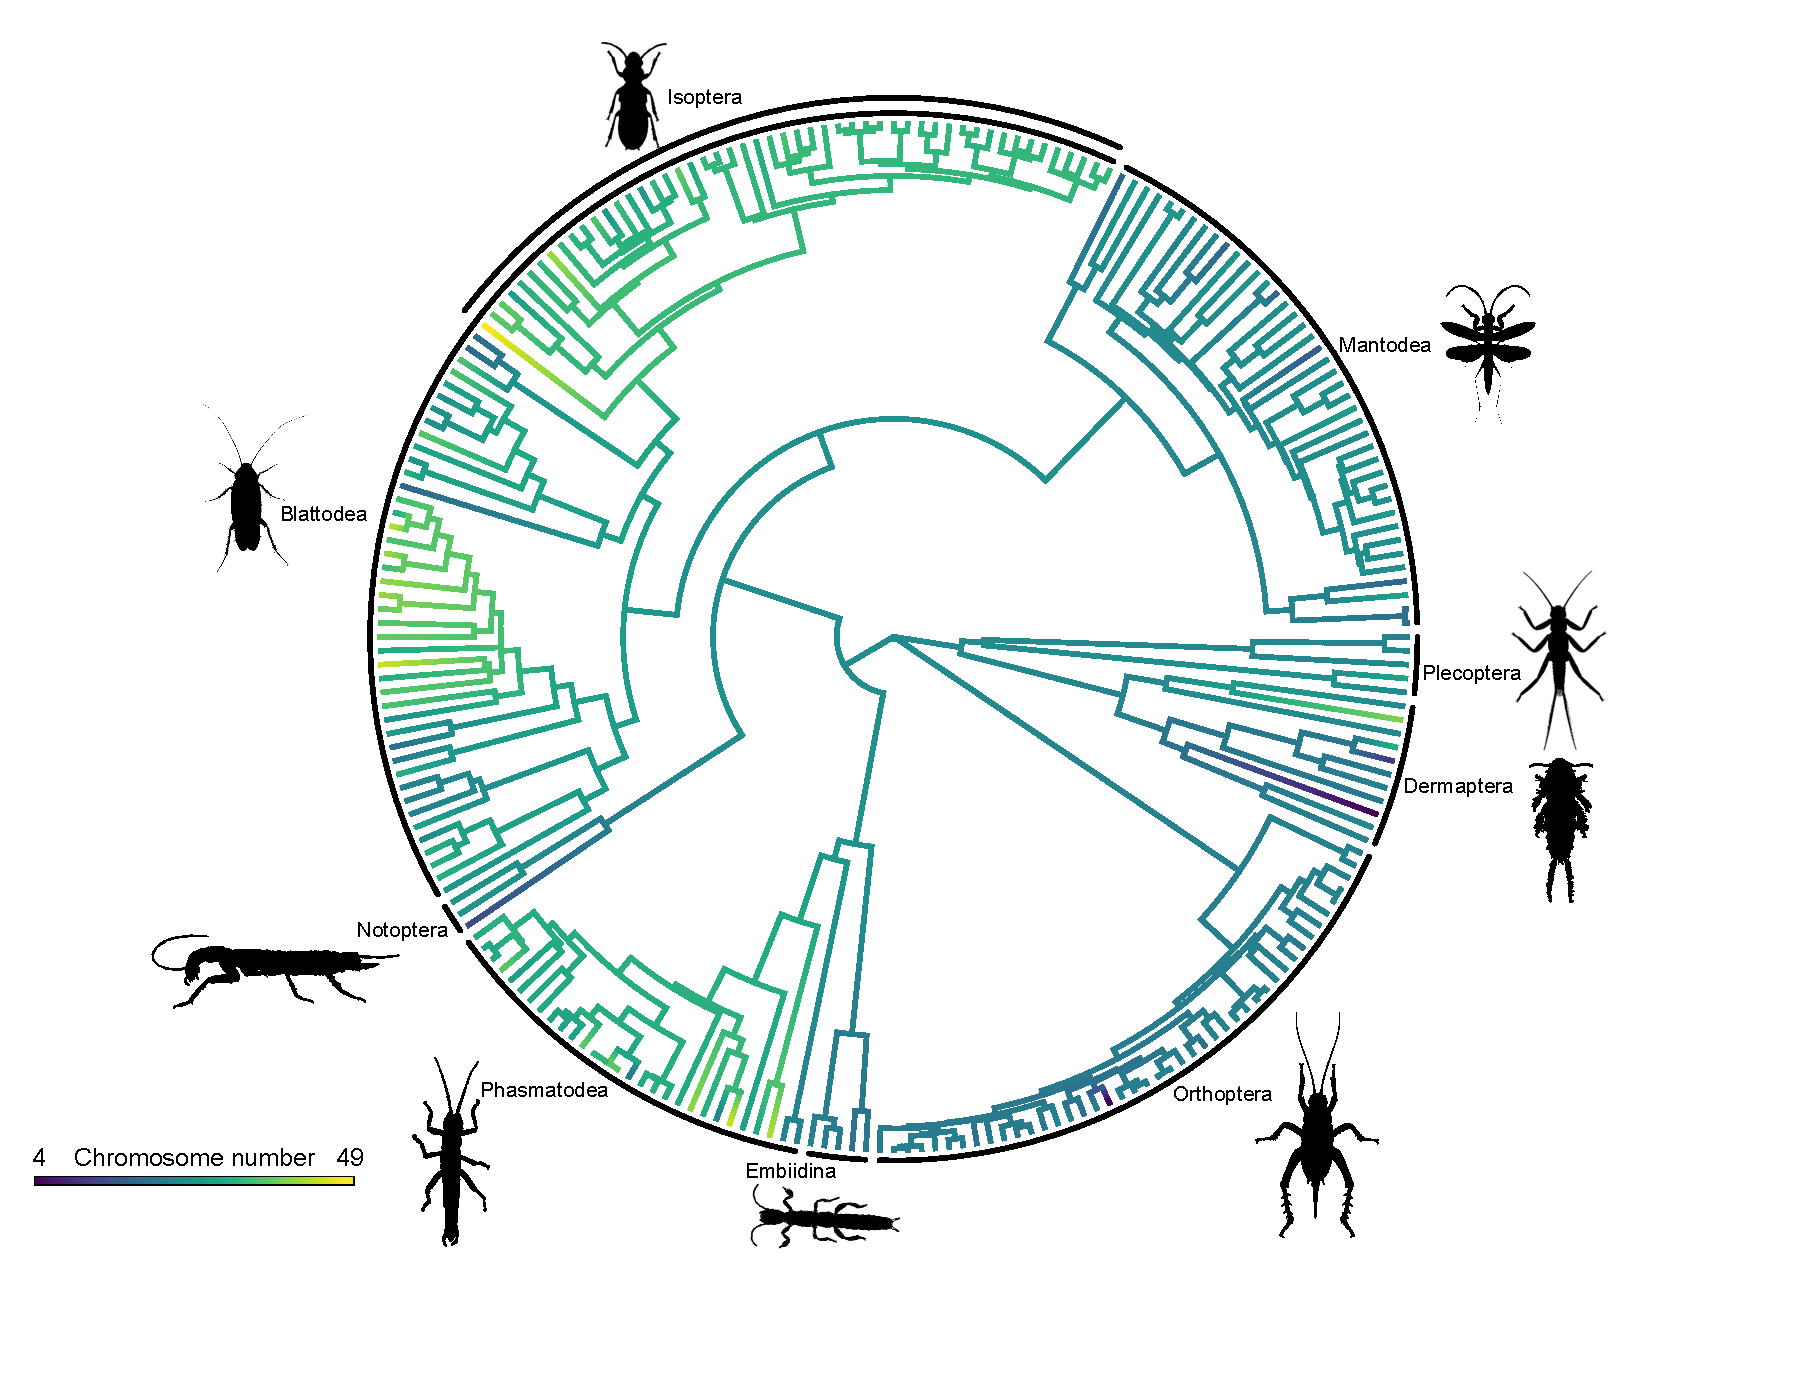
\includegraphics[width=1\textwidth]{figures/phylogenetic_tree.pdf}
\caption{
One of the 100 posterior distribution of trees giving a visual representation of the phylogenetic relationship of the orders in the Polyneoptera clade. The solid black line indicates the taxa for that perticular order. Isoptera is included within Blattodea as it has been identified as a highly derived clade within Blattodea. Branches are coloured according to the chromosome number of that lineage. 
}
\label{fig:phyloplot}
\end{figure}

\newpage
\begin{figure}
\centering 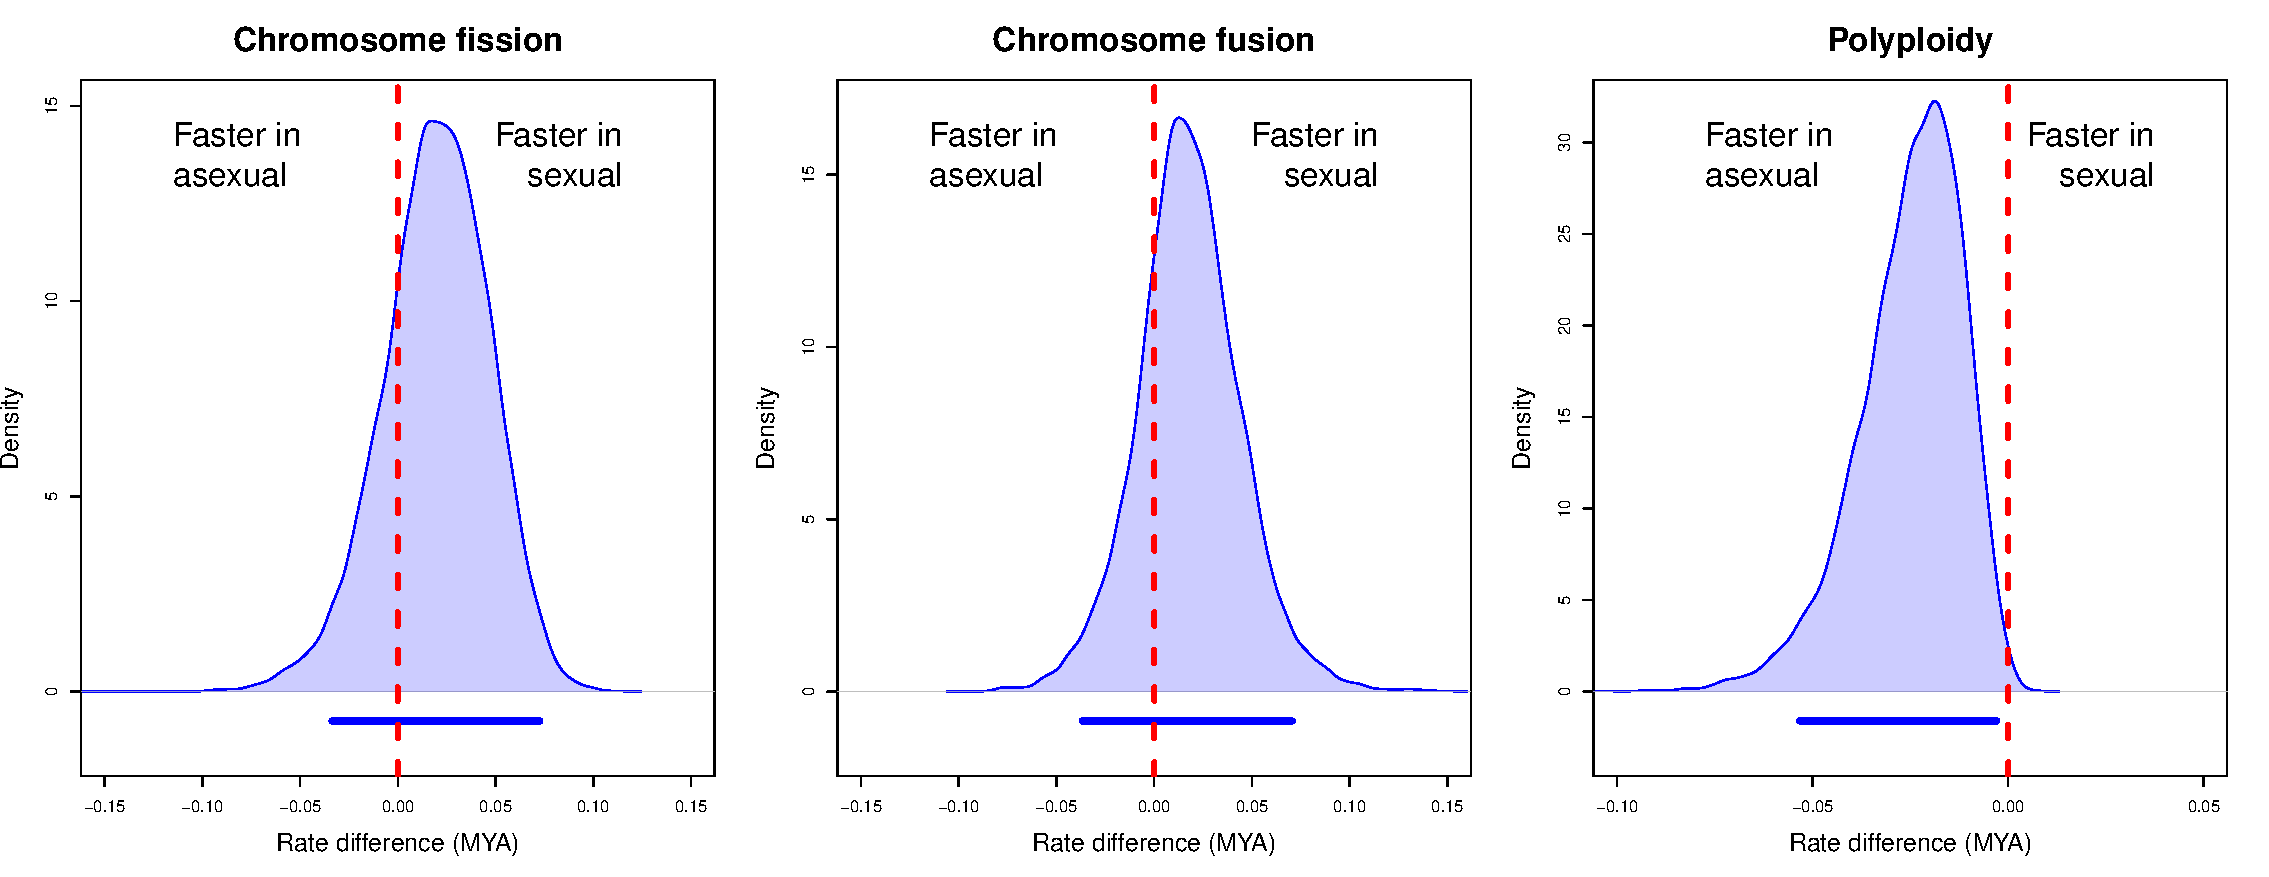
\includegraphics[width=.7\textwidth]{figures/phasmatodea_sex_asex_plot.pdf}
\caption{Chromosome evolution rates in sexual and asexual reproducing systems in the order Phasmatodea. Bars below the plot indicates the 95\% HPD interval}
\label{fig:phas.plot}
\end{figure}

\newpage
\begin{figure}
\centering 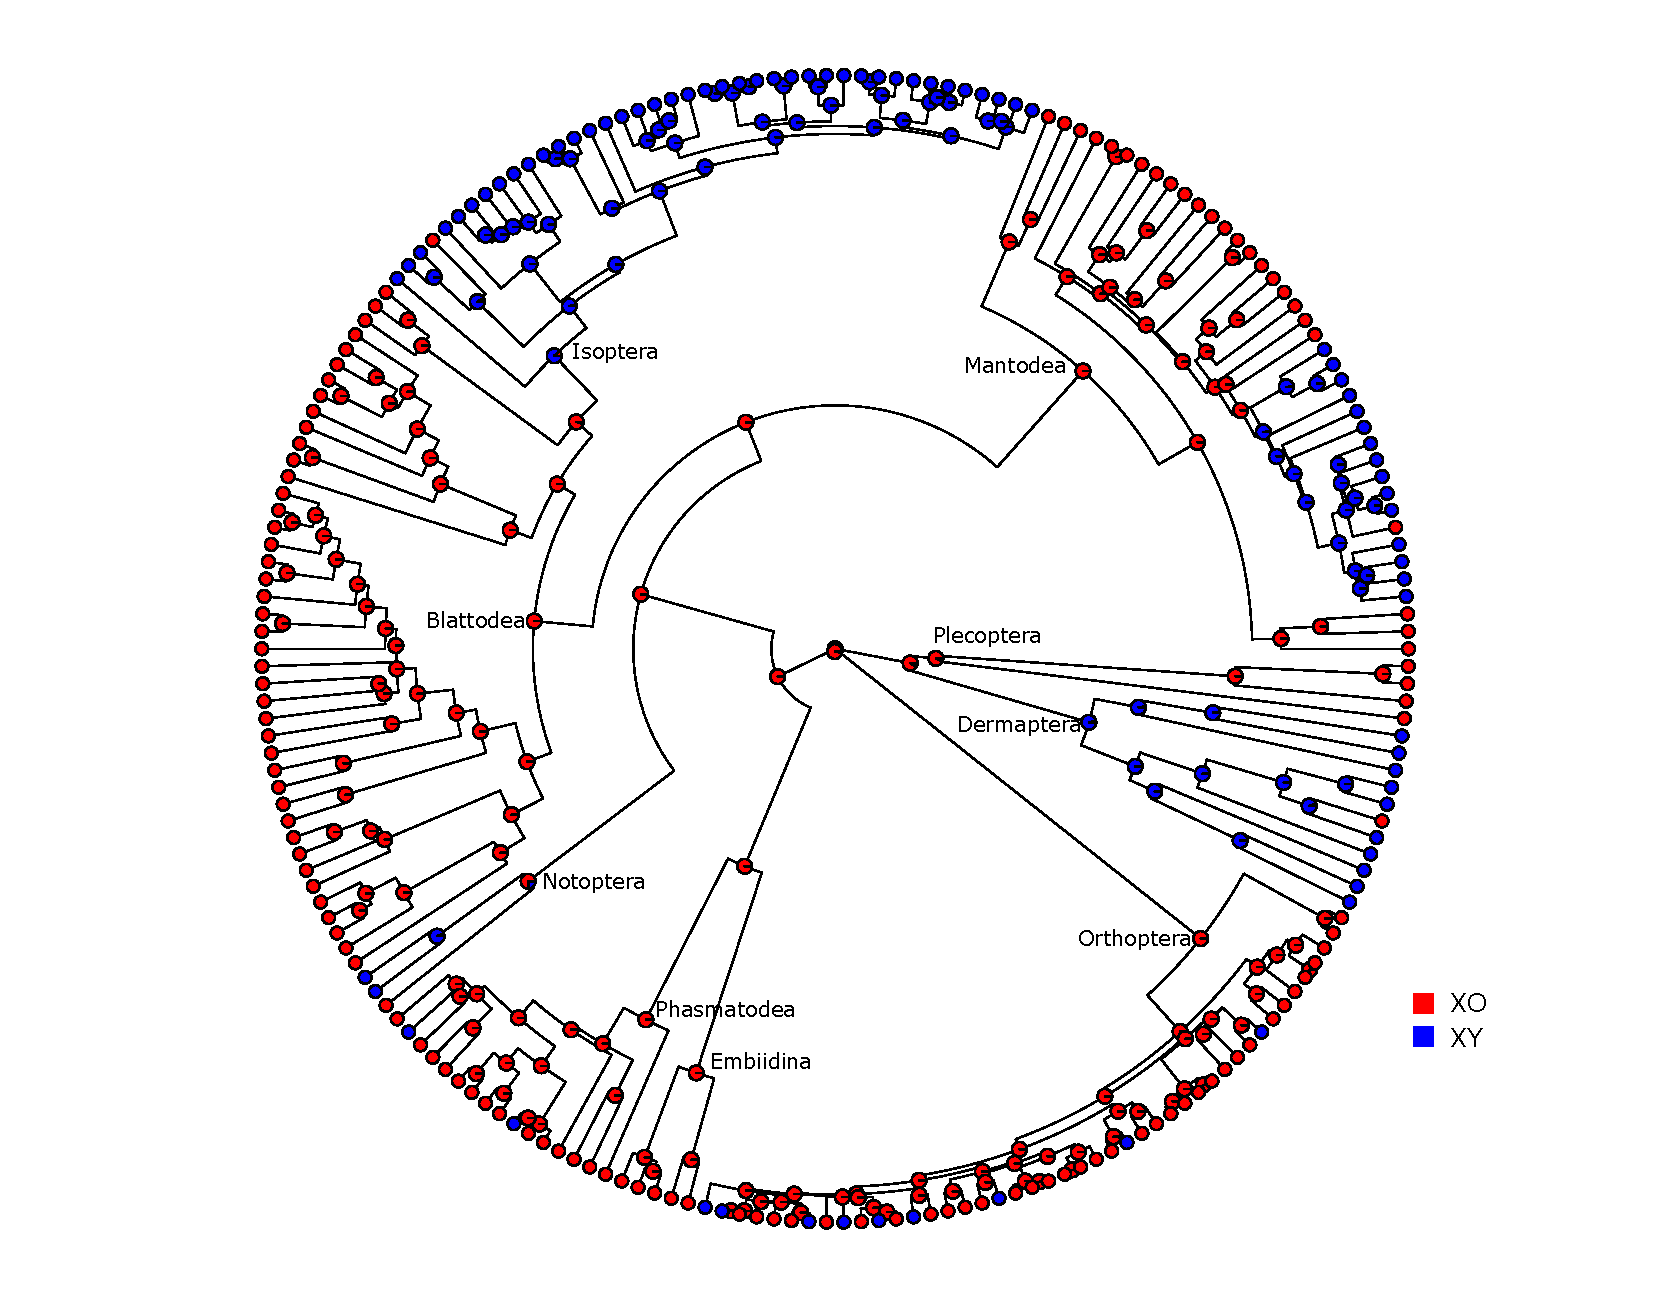
\includegraphics[width=1\textwidth]{figures/sex_chrom_asr_phylogeny.pdf}
\caption{Ancestral states reconstruction of the sex chromosome systems. This is a single tree of the posterior distribution. Red colour represents XO sex chromosome system and Blue colour represents XY sex chromosome systems. Order names are marked at the origin of each order. The probabilities of each sex chromosome system as being the ancestral state is given by the respective coloured potion of the pi charts at each node. Tip colours represent the current state of the sex chromosome system.}
\label{fig:sex.asr.plot}
\end{figure}

\newpage
\begin{figure}
\centering 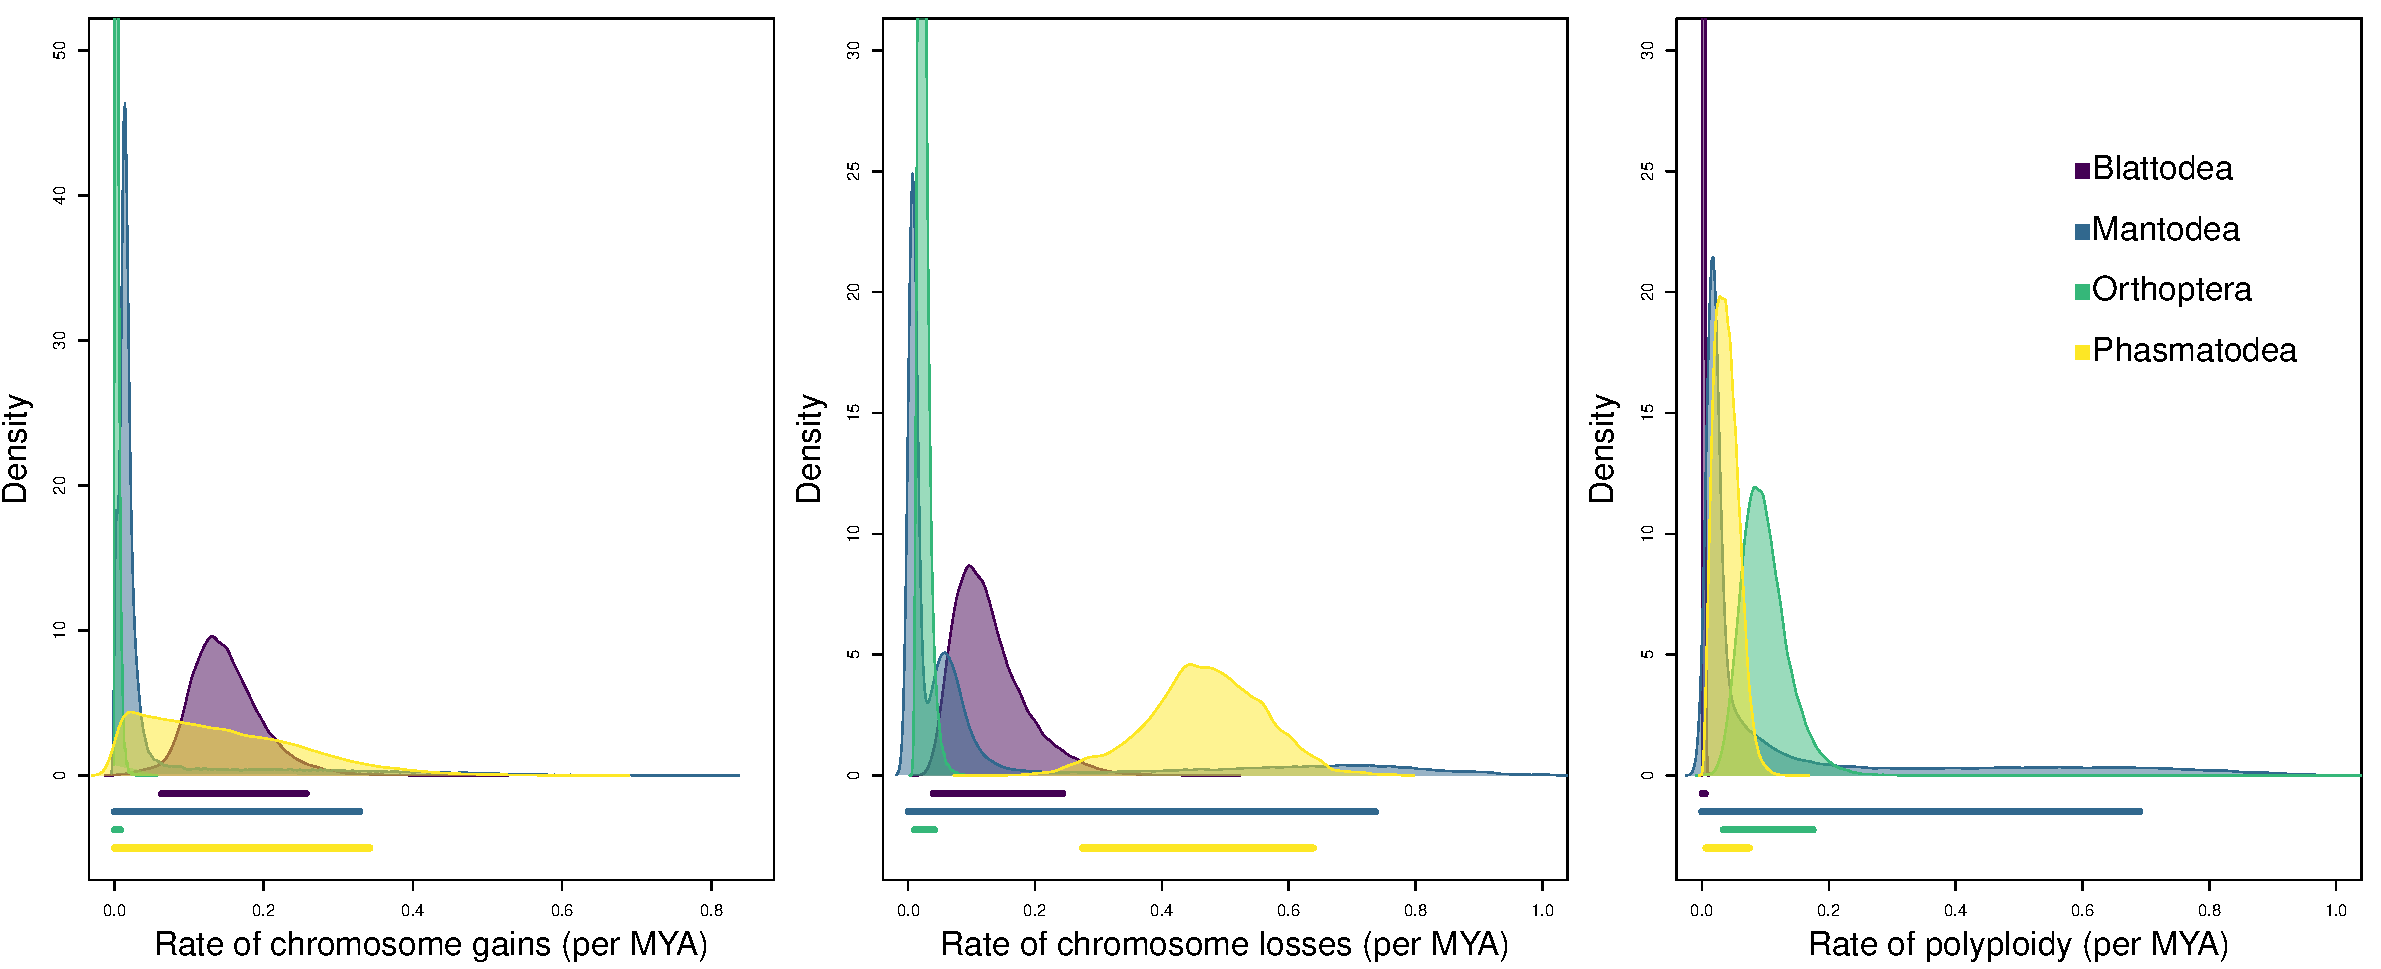
\includegraphics[width=.7\textwidth]{figures/order_rates_95HPD.pdf}
\caption{Rates of chromosome fusion, fission and, polyploidy of four orders in the insect clade Phasmatodea. The y axis is shortened to show the spread of these rates. The bars below each distribution indicates the 95\% HPD interval}
\label{fig:order.rates.95HPD}
\end{figure}

